\documentclass[11pt]{article}

\usepackage{latexsym}
\usepackage{graphicx}
\usepackage{amssymb}
\usepackage{amsthm}
\usepackage{enumerate}
\usepackage{amsmath}
\usepackage{cancel}
\numberwithin{equation}{section}
\numberwithin{figure}{section}
\numberwithin{table}{section}

\setlength{\evensidemargin}{.25in}
\setlength{\oddsidemargin}{-.25in}
\setlength{\topmargin}{-.75in}
\setlength{\textwidth}{6.5in}
\setlength{\textheight}{9.5in}
\newcommand{\due}{April 8th, 2010}
\newcommand{\HWnum}{9}
\newcommand{\grad}{\bold\nabla}
\newcommand{\vecE}{\vec{E}}
\newcommand{\scrptR}{\vec{\mathfrak{R}}}
\newcommand{\kapa}{\frac{1}{4\pi\epsilon_0}}
\newcommand{\unit}[1]{\ensuremath{\, \mathrm{#1}}}

\begin{document}
\begin{titlepage}
\setlength{\topmargin}{1.5in}
\begin{center}
\Huge{Physics 3320} \\
\LARGE{Principles of Electricity and Magnetism II} \\
\Large{Professor Ana Maria Rey} \\[1cm]

\huge{Homework \#\HWnum}\\[0.5cm]

\large{Joe Becker} \\
\large{SID: 810-07-1484} \\
\large{\due} 

\end{center}

\end{titlepage}



\section{Introduction}
We learned in previous labs that digital logic circuits can be very useful, but they become very complicated very quickly. A simpler solution to this problem is to use a microcontroller rather than building your circuit from scratch. A microcontroller is an integrated circuit that can be programmed. This allows for robust digital circuits to be built quickly and cheaply.

\section{Theory}
At a base level all digital circuits operate at a binary level. That is with ones and zeros or true and false. All digital logic is done at this level. So the commands and stored variables are actually seen by the mircocontroller as a binary number, where each 1 or 0 is called a \emph{bit} of data. It is very difficult for humans to interpret these values and well as the fact that binary numbers become very long. To remedy this we developed a hexadecimal system to represent the memory allocation of the microcontroller. A hexadecimal values are represented by the numbers 0 through 9 and the letters a through f. Where f is 15 in a base 10 system. So we see that each hexadecimal value represents 4 digits of binary. We call this a \emph{byte} of data.

Now, this does not make the instructions on the microcontroller easier to understand. We still have numbers and we usually like to read words. This is where the assembly programing language comes in. This is a basic language that allows us to define variables with names that we can set a value to. This also allows us to create and name commands that we can call in the program. This is the basics of computer programing. While assembly works just like more complex and robust programming languages, it is still very limited in what is possible. Also the specific commands and input/output variables vary from microcontroller to microcontroller. Also the microcontroller cannot interpret the assembly code on its own. The code needs to be converted into hexadecimal so the microcontroller can interpret the commands. This requires the use of a assembler that needs to be run on a separate system usually another external computer.

\section{Experiment}
For this lab the microcontroller we used was the PIC16F676 or the PICChip. An important feature of the PIC16F676 is that we can connect the microcontroller to a computer's universal serial bus through the PICkit. The PICkit is another integrated circuit that can be used to power the microcontroller as well as upload the Hex code onto the IC itself. So to begin we connected the PIC16F676 to the PICkit as shown in figure \ref{FigSchem}
\begin{figure}[h]
\centering
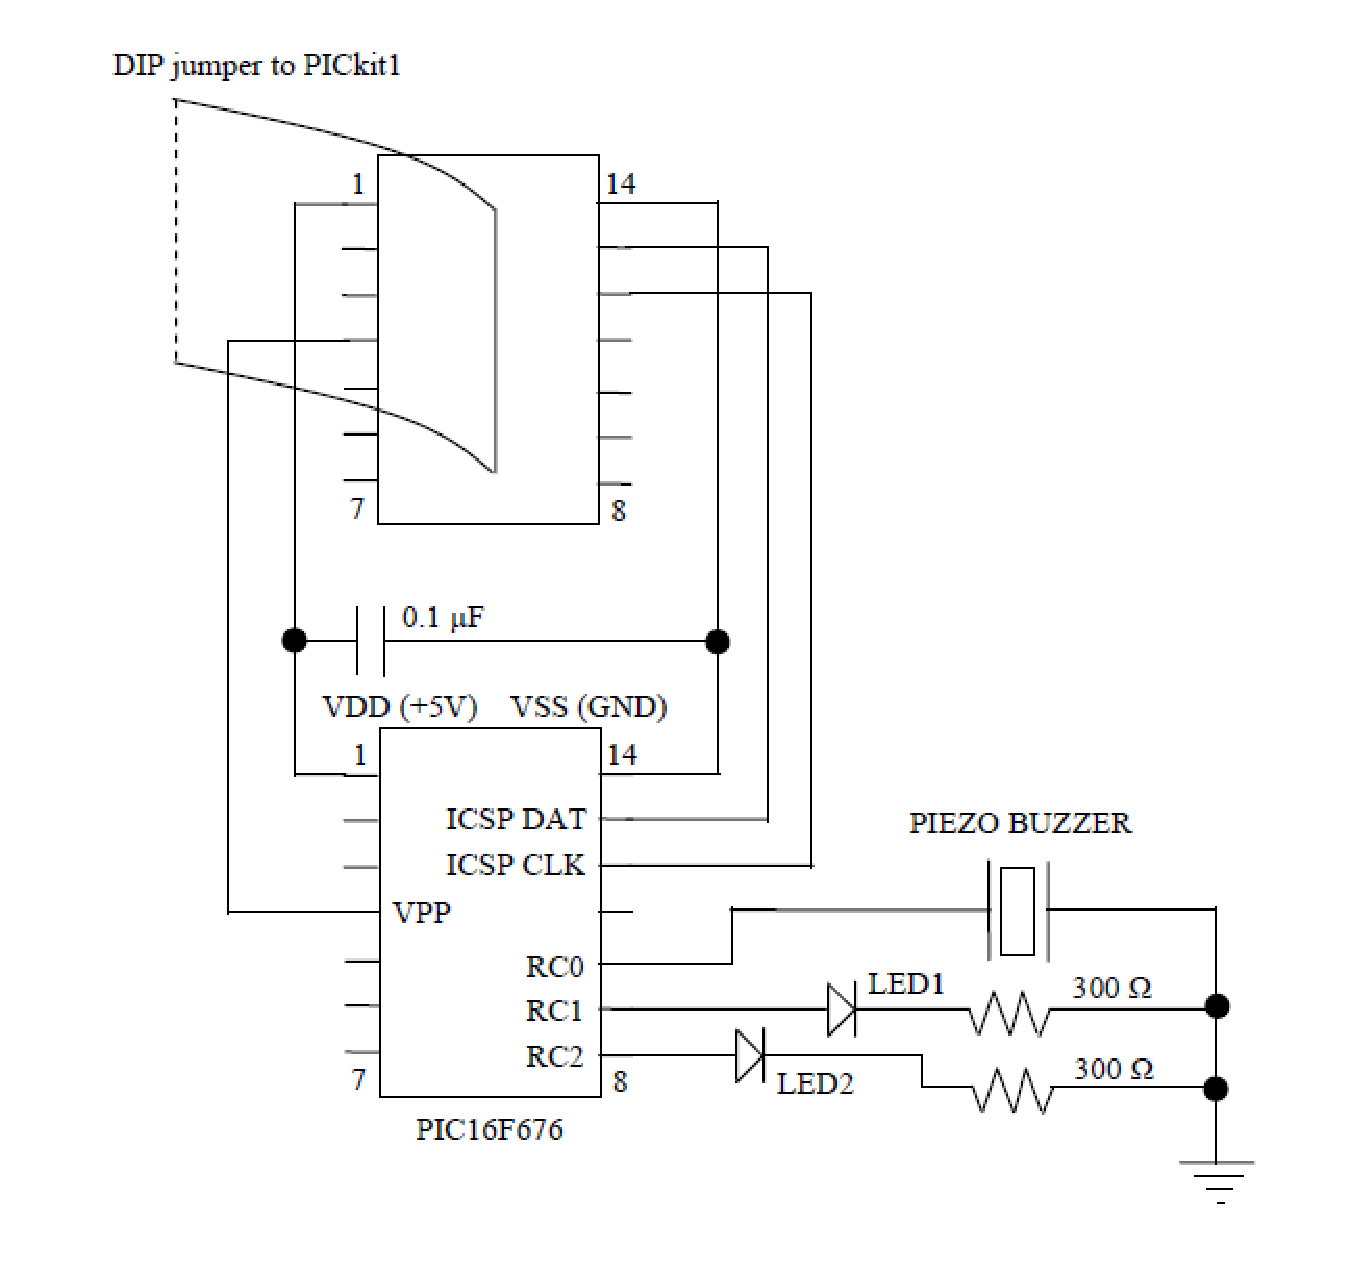
\includegraphics[scale=0.60]{FigSchem.eps}
\caption{\textit{The circuit for the alarm. Note that the capacitor across the input voltage is prevent any voltage jumps.}}
\label{FigSchem}
\end{figure} 

Once the circuit in figure \ref{FigSchem} was built we connected the USB from the PICkit to a computer. We then downloaded the sample code. The man purpose of this code is to turn the buzzer on and off and turn the LEDs on and off. We opened the sample code in the MPLAB IDE program. Using this program we converted the assembly code into a Hex file. We then used the PICkit software to upload the hex file to the PIC16F676. We ran the program and it behaved as we expected. Then we modified the sample program so that the buzzer will beep two different frequencies (tones) in an alternating pattern and the LEDs will alternate off and on. So one LED is on while the other is off, then they switch. This will loop forever. Again we converted the assembly code to a hex file using the MPLAB IDE program and we uploaded the code to the microcontroller and it ran as we expected. See attached for the modified assembly code.


\section{Conclusion}
Often in physics experiments we need to make a quick and dirty logical circuit. A microcontroller is a simple and cheap solution to this problem. As we have seen a microcontroller allows the user to make a custom circuit just by programing the IC.
\end{document}

